% ---------------------------------------------------
% ----- Chapters of the template
% ----- for Bachelor-, Master thesis and class papers
% ---------------------------------------------------
%  Created by C. Müller-Birn on 2012-08-17, CC-BY-SA 3.0.
%  Freie Universität Berlin, Institute of Computer Science, Human Centered Computing. 
%
\chapter{Umsetzung}
\label{chap:implementation}
		
		Die im Rahmen dieser Masterarbeit entwickelte Software besteht aus einem
		modularen Kern und ist über verschiedene Technologien ansprechbar. Aktuell
		sind die Matcher als App
		für Django\footnote{\url{https://www.djangoproject.com/}} verfügbar, können
		aber auch direkt in Python Skripten benutzt werden.\\
		Der Kernteil besteht aus mehreren Modulen, für die weitere Module
		implementiert werden können, um verschiedene Arten von Daten eingelesen
		werden können, z.B.
		Formate wie OWL/XML, Query Languages wie SPARQL oder REST-Schnittstellen.
		Zusätzlich können unterschiedliche Arten und Implementierungen von Matchern
		verwendet werden. Um dies zu realisieren, gibt es eine Klasse, um Ontologien,
		deren Elemente und Eigenschaften abzubilden, namens \textit{ontology}.
		Die Elemente dieser Instanzen bestehen wiederum aus Instanzen der Klasse
		\textit{onto element}. Dort enthalten sind alle Informationen, die das Element
		beschreiben. Diese beiden Klassen dienen als Schnittstellen, um innerhalb der
		Software mit Ontologien und deren Elementen zu interagieren.
		
		\section{Architektur}
		Sowohl die Kernmodule als auch die einzelnen, konkreten Ausführungen dieser
		Module sind entlang eines Prozesses organisiert, wie in Abbildung \ref{fig2}
		gezeigt.
		\begin{figure}[ht]
		\centering
		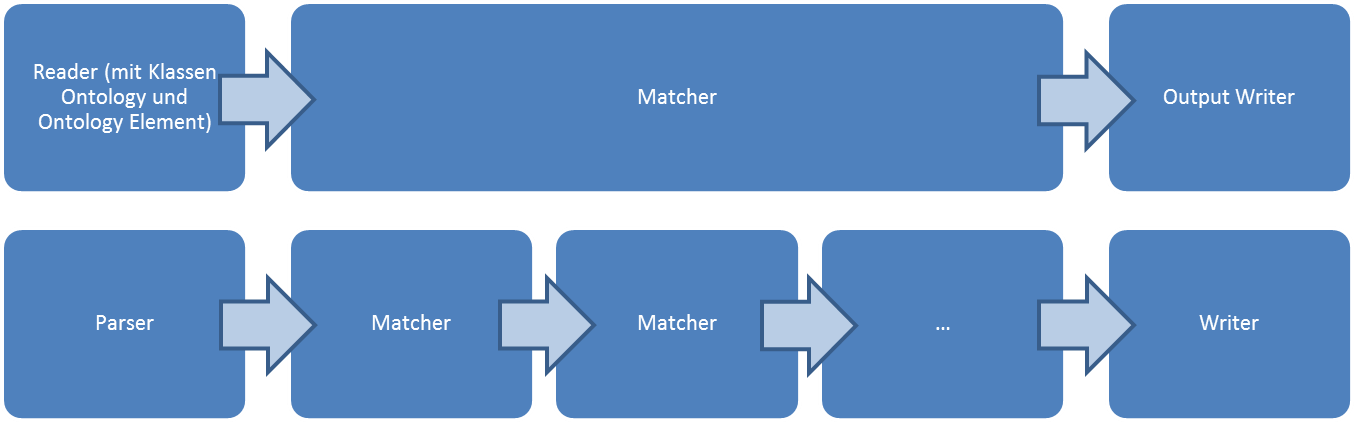
\includegraphics[width=1.0\textwidth]{pics/Module-overview.png}
		\caption{Prozessablauf der Module}
		\label{fig2}
		\end{figure}
		An erster Stelle stehen der oder die Parser, die die Ontologien einlesen und
		die Daten in Instanzen der Klasse \textit{ontology} einpflegen. Hierbei können
		auch Daten aus unterschiedlichen Quellen und beliebigen Formaten verwendet
		werden, sofern ein \textit{Reader} implementiert wurde. Im Rahmen dieser
		Masterarbeit wurden bereits einige implementiert, die einige gängige
		Möglichkeiten abdecken. Durch die Modularität können aber problemlos weitere
		hinzugefügt werden.\\
		Dann werden die Ontologien an verschiedene Matcher übergeben. Dabei werden
		die Ergebnisse von einem Matcher zum nächsten weitergegeben, so ist es zum
		einen möglich, diese Ergebnisse zu akkumulieren und zum
		anderen, weitergehende Analysen z.B. der Struktur oder Hierarchie vorzunehmen.
		Die Gesamtergebnisse werden dann an einen \textit{Output Writer} übergeben, um
		sie dann weiter bearbeiten zu können.\\
		
		
		\subsection{Anwendungsszenario 1: Django App}
		Wenn die Module der Matching Software als Teil einer Django App genutzt
		werden, werden über ein
		Skript\footnote{SimpleOntologyMatcher/OntologyMatcher/settings.py} von Django
		mögliche Ontologien und Matcher gesammelt.
		
		\begin{figure}[ht]
		\centering
		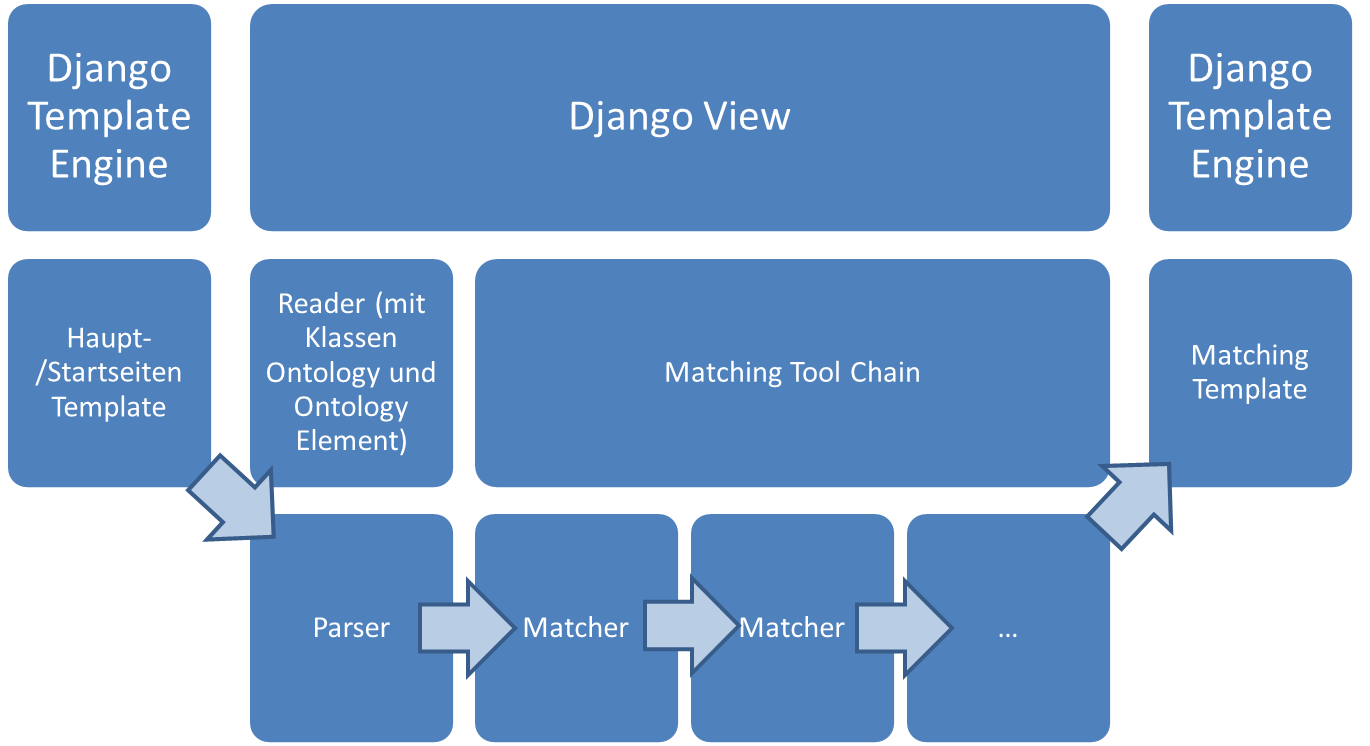
\includegraphics[width=1.0\textwidth]{pics/Module-overview1.png}
		\caption{Module Django App}
		\label{fig6}
		\end{figure}
		Dabei können, wie erwähnt, verschiedene Quellen verwendet werden. Für
		Ontologien sind lokale und auf externen Servern gespeicherte Dateien und in Datenbank
		eingepflegte Daten möglich. Bei Matchern werden nur lokal vorhandene Python
		Module berücksichtigt. Die gefundenen Ontologien und Matcher werden dann in
		ein HTML Template eingebetet, dass mit der textit{Django Template Engine} erstellt wird. Dabei wird auch die Quelle gespeichert, also der Dateiname mit Pfad oder
		die URL.\\
		Über die dann erstellte Seite können Ontologien ausgewählt werden, die
		analyisert werden sollen, und Matcher, mit denen dies durchgeführt wird.\\
		Das Design ist möglichst simpel gewählt, wie in \ref{fig3} gezeigt. Dadurch
		wird die Bedienung und gleichzeitig die Komplexität zu verringert, da die
		Optionen und Bedienung limitiert sind. Die GUI ist auf das Nötigste
		reduziert und nicht überfrachtet. Ein einfaches User Interface hilft auch bei
		der Akzeptanz, da der Einstieg ohne Vorkenntnisse auch für Fachfremde Personen
		erleichtert wird.
		
		\begin{figure}[ht]
		\centering
		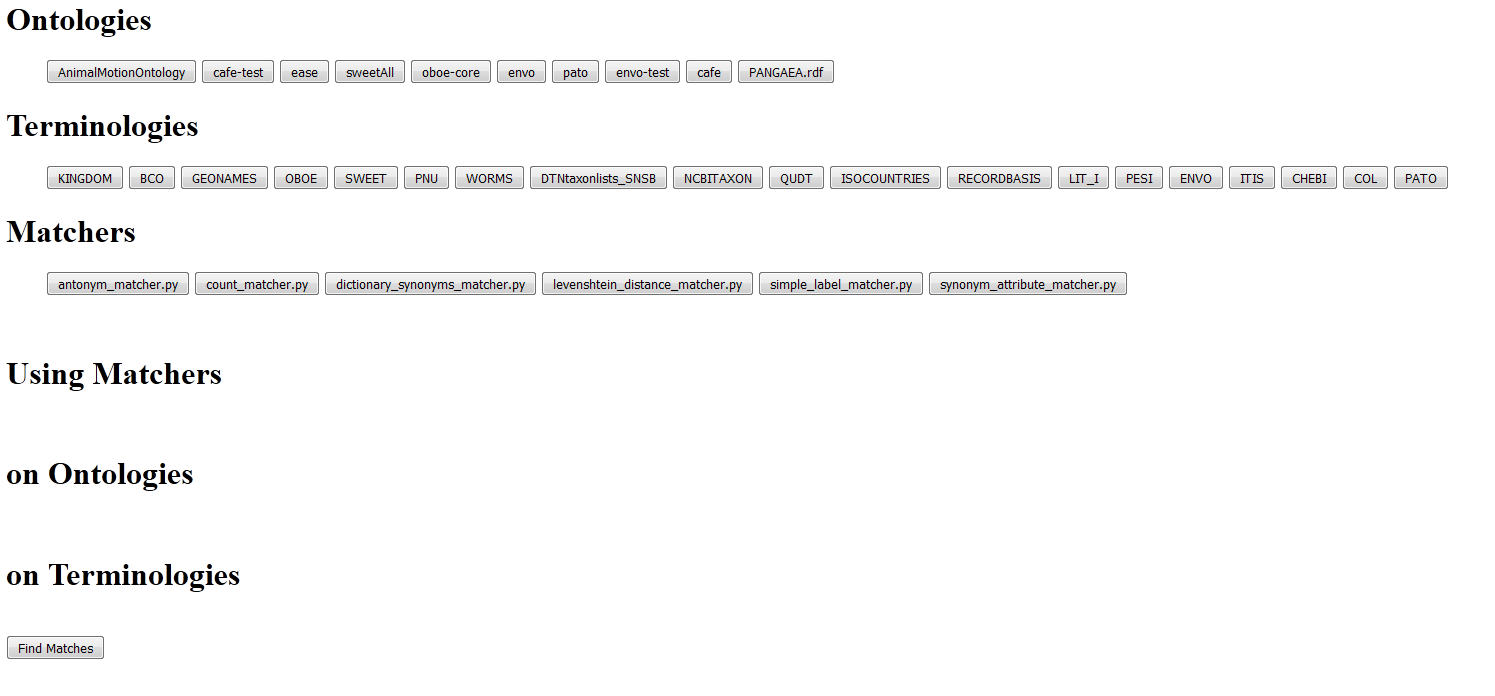
\includegraphics[width=1.0\textwidth]{pics/TemplateMatchingStartPage.png}
		\caption{Startseite Django App 1}
		\label{fig3}
		\end{figure}
		Wenn sowohl Ontologien bzw. Terminologien als auch mindestens ein Matcher
		gewählt wurden, wird der Matching Prozess, wie in \ref{fig4} gezeigt,
		gestartet.
		
		\begin{figure}[ht]
		\centering
		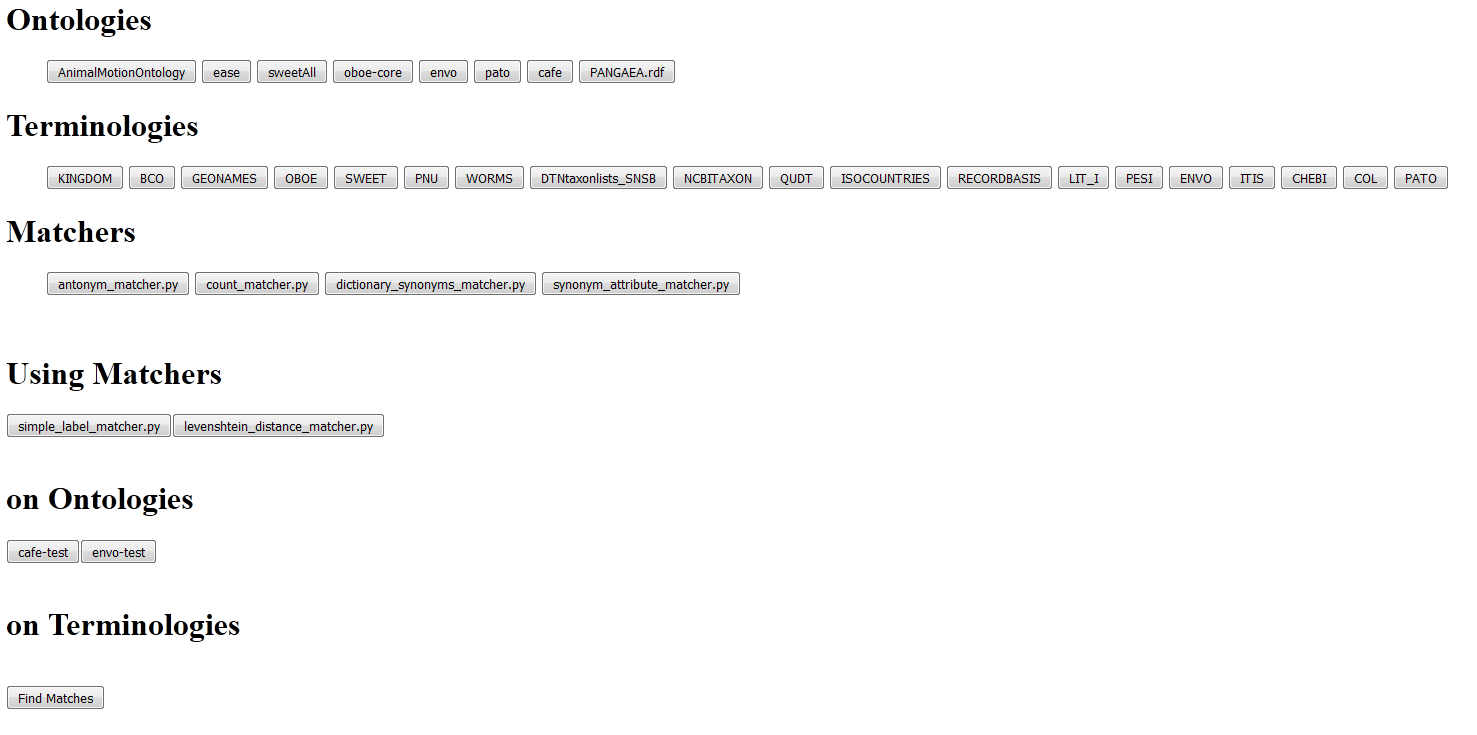
\includegraphics[width=1.0\textwidth]{pics/TemplateMatchingStartPage1.png}
		\caption{Startseite Django App 2}
		\label{fig4}
		\end{figure}
		Anschließend werden die ausgewählten Ontologien mit entsprechenden
		\textit{Readern} geparst. Die Reader werden ermittelt, indem überprüft wird,
		ob es sich bei der gespeicherten Quelle um eine URL oder eine
		existierende Datei handelt. Dies wird über das \textit{View} von Django
		erledigt und dann an das \textit{Reader} Modul weitergeleitet. Dieses bindet
		die passenden Module ein, startet das Parsen und liefert die Ergebnisse
		zurück. Die Ergebnisse bestehen aus Instanzen des Moduls \textit{onto} in
		einer Liste.\\
		Mit den übergebenen Matchern wird eine \textit{Matching Tool Chain} im
		gleichnamigen Modul erstellt, welche die Matcher in der angegebenen
		Reihenfolge ausführt. Die Ergebnisse jedes Matching Vorgangs werden von einem
		Matcher an den nächsten in Form des Python Datentyps \textit{Dictionary}
		weitergegeben. Dadurch ist es möglich, auf vorherige Ergebnisse zuzugreifen,
		um z.B. die Struktur zu analysieren. Die eigenen Ergebnisse eines Matchers
		werden einfach zum Dictionary hinzugefügt.\\
		Wenn alle Matcher durchlaufen wurden, wird das letztendliche Ergebnis in einem
		anderen Template der Django Template Engine verarbeitet und angezeigt,
		wie in \ref{fig5} exemplarisch dargestellt.
				
		\begin{figure}[ht]
		\centering
		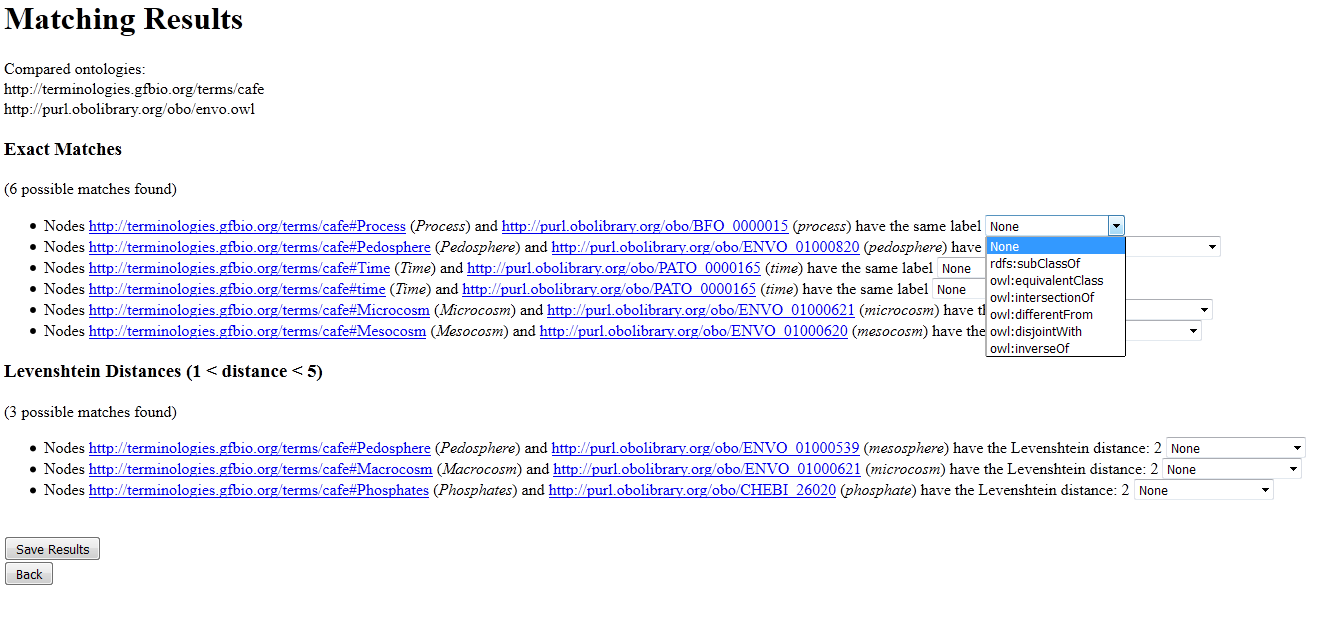
\includegraphics[width=1.0\textwidth]{pics/TemplateMatchingResultPage.png}
		\caption{Django App Resultatseite}
		\label{fig5}
		\end{figure}
		Auf dieser Seite kann dann gewählt werden, ob zwei Elemente eine Verbindung
		haben und welche dies ist. Wenn allen Paaren von Elementen eine Art von
		Verbindung oder eben keine zugeordnet wurde, ist es möglich, das Ergebnis in
		eine Datei im XML Format zu exportieren.
		
		\subsection{Anwendungsszenario 2: Python Skript}
		Neben der Möglichkeit den Simple Ontology Matcher als Django App zu verwenden,
		können die einzelnen Module auch wie üblich als normale Python Module
		importiert und aufgerufen werden. Dabei ist es möglich, die Module der
		Zwischenschicht\footnote{matcher.py und reader.py} zu verwenden oder
		auszulassen, da diese nur das dynamische Einbinden übernehmen.
		
		\section{Implementierte Matcher}
		Im Rahmen dieser Masterarbeit wurden verschiedene Matching Algorithmen
		implementiert. Das Ziel der verschiedenen Matcher ist nicht nur Beziehungen,
		die Gleichheit oder Ähnlichkeit ausdrücken, zu finden, sondern möglichst
		verschiedene Arten von Verknüpfungen.
		
		\subsection{Same Entity Matcher}
		Der einfachste Matcher überprüft die URI der Elemente, um festzustellen, ob es
		in den übergebenen Ontologien gleiche Elemente gibt. Dies wird über eine
		einfach Abfrage auf Gleichheit der gesicherten URIs getan.
		\begin{lstlisting}
		for i in onto_elements:
			for j in onto1_elements:
				if re.match(i.name, j.name, re.IGNORECASE):
		\end{lstlisting}
		
		\subsection{Simple Label Matcher}
		Bei diesem Matcher werden die Labels der Elemente auf Ähnlichkeiten
		untersucht.
		Zuerst werden die Labels auf Gleichheit überprüft.
		\begin{lstlisting}
		match_result = re.match("^" + item.get_text() + "$", item1.get_text(), re.IGNORECASE)
		if not already_matched and match_result and not re.match(i.name, j.name, re.IGNORECASE):
		\end{lstlisting}
		Anschließend wird einfach nach Übereinstimmungen in den Labels gesucht.
		\begin{lstlisting}
		elif not already_matched and ((re.match(item.get_text(), item1.get_text(), re.IGNORECASE) and len(item.get_text()) > 3) or (re.match(item1.get_text(), item.get_text(), re.IGNORECASE) and len(item1.get_text()) > 3)) and not re.match(i.name, j.name, re.IGNORECASE):
		\end{lstlisting}
		Die reguläre Ausdrucküberprüfung wird in beide Richtungen durchgeführt, da in
		der Python re.match Funktion der im ersten Argument übergebene Ausdruck im
		zweiten gesucht wird. In beiden Fällen darf der gesuchte Ausdruck aber nicht
		kürzer als vier Zeichen sein. In früheren Tests, wo es diese Einschränkung
		noch nicht gab, waren in der Ergebnismenge viele false positives.
		Die erste Bedingung in beiden Abfragen ist nach der Variable
		\textit{already\textunderscorematched}, diese dient dazu festzuhalten, ob zwei Elemente
		bereits als mögliches Matching vorgemerkt wurde. Dies ist für den Fall
		gedacht, dass es mehr als ein Label für ein Element gibt. Sollte dies
		vorkommen, werden nicht alle Kombinationen von Labels überprüft, falls es
		bereits bei einem Paar ein Treffer gab. Dadurch können potenziell Vergleiche
		und damit Zeit eingespart werden.
		
		\subsection{Levenshtein Distance Matcher}
		Dieser Matcher berechnet die Levenshtein Distanz bzw. den Editierabstand
		zwischen den Labeln zweier Elemente. Also wie viele Änderungen der Buchstaben
		man an einem Label durchführen muss, um das andere Label zu erhalten.\\
		Zuerst wird geprüft, ob beide Label aus mehr als drei Buchstaben bestehen.
		Dann wird der Abstand, ob der Abstand zwischen beiden berechnet. Damit ein
		Elementenpaar als mögliches Matching anerkannt wird, muss der Abstand größer
		als eins und kleiner als fünf sein. Zusätzlich darf der Abstand nicht größer
		als ein Drittel der Länge beider Label sein.\\
		In der ersten Version dieses Matchers war die einzige Bedingung, dass der
		Editierabstand größer als eins und kleiner als fünf sein musste.
		\begin{lstlisting}
		if 1 < distance and distance < 5 and (distance < len(item.get_text())/3) and not already_matched:
		\end{lstlisting}
		Probleme traten bei kurzen Wörtern, da dann alle Buchstaben geändert werden
		konnten. Aus diesem Grund wurden die Bedingungen eingeführt, dass mehr als ein Buchstabe
		geändert werden muss und die Veränderungen maximal ein Drittel der Buchstaben
		umfassen dürfen (siehe auch \ref{subsec:Evaluation 1} Evaluation 1).
		\begin{lstlisting}
		if not already_matched and 1 < distance and distance < 5 and (distance < len(item.get_text())/3) and (distance < len(item1.get_text())/3) and not re.match(i.name, j.name, re.IGNORECASE):
		\end{lstlisting}
				
		\subsection{Dictionary Synonym Matcher}
		Mit diesem Matcher werden über die PyDictionary
		API\footnote{\url{https://pypi.python.org/pypi/PyDictionary}} Synonyme der
		Labels abgefragt und diese mit den anderen Labels verglichen. Sobald es eine Übereinstimmung in den Synonymen eines Labels mit einem anderen gibt, wird
		dieses Elementenpaar als mögliches Matching vorgemerkt.\\
		Bei diesem Matcher hat sich der Kontext der Ontologie als Schwachstelle
		herausgestellt, da viele Begriffe verschiedene Bedeutungen haben, insbesondere
		in bestimmten Wissenschaften. Dann ergeben viele Synonyme keinen Sinn.\\
		Ein weiteres Problem dieses Matchers ist die Laufzeit, da die Dauer Anfrage
		zusammen mit der Menge der Anfragen den gesamten Prozess spürbar in die Länge
		ziehen. Eine mögliche andere Quelle für einen derartigen Matcher ist daher
		wünschenswert.
		
		\subsection{Dictionary Antonym Matcher}
		Bei diesem Matcher werden analog zum \textit{Dictionary Synonym Matcher}
		Antonyme, also Gegenteile von Wörtern, betrachtet.
		
		\subsection{Synonym Matcher}
		Um das Problem mit den Synonymen anzugehen, wurden bei der German Federation
		for Biological Data (GFBio)\footnote{\url{http://www.gfbio.org}} Synonyme als
		Eigenschaft eingeführt. Dieser Matcher bedient sich dieser Synonyme, um nach passenden
		Matchings zu suchen. Die verringert auch die 
		
		\section{Sicherheit}
		Sicherheit ist bei der Softwareentwicklung ein wichtiger Aspekt, der
		betrachtet werden muss. Dies gilt insbesondere bei einer Webanwendung, da
		dort mit Eingaben von Außen gearbeitet wird. Außerdem sind der Nutzerkreis
		nicht eingeschränkt und Nutzer nicht per se bekannt.
		
		\subsection{XML}
		Daten, die in XML vorliegen, lassen sich grundsätzlich so gestalten, dass sie
		schädliches Verhalten hervorrufen. Denkbar sind
		\textit{Denial of Service} (DoS) Attacke, Zugriff auf lokale Dateien,
		Erstellen von Netzwerkverbindungen oder Umgehung von
		Schutzmaßnahmen.\footnote{\url{https://docs.python.org/2/library/xml.html#xml-vulnerabilities}}
		Das Modul aus der Python Standardbibliothek, um XML Dateien bzw. XML
		formatierte Strings zu lesen, ist gegen derartige Angriffe nicht explizit
		geschützt. Es gibt zwei Bibliotheken, die in der Dokumentation von Python 2
		erwähnt werden, die die Sicherheitsproblematik angehen (\textit{defused
		packages}).\footnote{\url{https://docs.python.org/2/library/xml.html#defused-packages}}
		Für den Simple Ontology Matcher wurde eine dieser beiden verwendet, defusedxml.\footnote{\url{https://pypi.python.org/pypi/defusedxml}} Dadurch
		soll die Möglichkeit verringert werden, dass der Simple Ontology Matcher als
		Einfallstor für Schadsoftware dient.
		
		\subsection{Exponential Entity Expansion}
		Bei dieser Art Angriff werden XML Entities benutzt, um den Inhalt einer
		einzulesenden XML Datei gezielt um ein Vielfaches zu vergrößern. XML Entities
		dienen dazu, Zeichen durch andere gezielt zu ersetzen. Bei einer
		für eine solche Attacke präpariertem XML werden rekursiv auszuführende
		Definitionen angelegt, die dann zu einer vielfachen Menge der angelegten
		Definition führen. Dadurch wird der Parser und eventuell auch das System, auf
		dem der Parser läuft, lahmgelegt, indem unerwartet eine große Menge
		Arbeitsspeicher belegt werden. Dieser Angriff ist auch als \textit{billion laughs} oder XML
		Bombe bekannt.\cite{Sul09} Ein Beispiel für solch einen Angriff ist hier aufgeführt:
		\begin{lstlisting}
		<?xml version="1.0"?>
		<!DOCTYPE lolz [
		 <!ENTITY lol "lol">
		 <!ELEMENT lolz (#PCDATA)>
		 <!ENTITY lol1 "&lol;&lol;&lol;&lol;&lol;&lol;&lol;&lol;&lol;&lol;">
		 <!ENTITY lol2 "&lol1;&lol1;&lol1;&lol1;&lol1;&lol1;&lol1;&lol1;&lol1;&lol1;">
		 <!ENTITY lol3 "&lol2;&lol2;&lol2;&lol2;&lol2;&lol2;&lol2;&lol2;&lol2;&lol2;">
		 <!ENTITY lol4 "&lol3;&lol3;&lol3;&lol3;&lol3;&lol3;&lol3;&lol3;&lol3;&lol3;">
		 <!ENTITY lol5 "&lol4;&lol4;&lol4;&lol4;&lol4;&lol4;&lol4;&lol4;&lol4;&lol4;">
		 <!ENTITY lol6 "&lol5;&lol5;&lol5;&lol5;&lol5;&lol5;&lol5;&lol5;&lol5;&lol5;">
		 <!ENTITY lol7 "&lol6;&lol6;&lol6;&lol6;&lol6;&lol6;&lol6;&lol6;&lol6;&lol6;">
		 <!ENTITY lol8 "&lol7;&lol7;&lol7;&lol7;&lol7;&lol7;&lol7;&lol7;&lol7;&lol7;">
		 <!ENTITY lol9 "&lol8;&lol8;&lol8;&lol8;&lol8;&lol8;&lol8;&lol8;&lol8;&lol8;">
		]>
		<lolz>&lol9;</lolz>
		\end{lstlisting}
		Dabei handelt es sich um valides und wohlgeformtes XML. Wenn ein XML Parser
		dieses XML Dokument lädt, wird das Element <lolz> gefunden, welches den Text
		“&lol9;” enthält. Dieses ist als Entität definiert, welches aus zehn mal der
		Zeichenkette “&lol8;” besteht. Dieses setzt sich aus zehn mal
		dem Ausdruck “&lol7;”  zusammen. Dies wird nun weitergeführt, bis alle
		Entitäten aufgedröselt wurden. Danach bestehen die Daten aus einer Milliarde
		mal dem Ausdruck "`lol"'. Daher auch die Bezeichnung billion laughs. Die Menge an
		Daten ist dadurch von weniger als einem Kilobyte auf fast drei GB
		angewachsen.\cite{Sul09}
		
		\subsection{Quadratic Blowup Entity Expansion}
		Dieser Angriff funktioniert ähnlich der Exponential Entity Expansion, nutzt
		aber keine Verschachtelung von Entitäten, sondern wiederholt eine sehr lange
		Zeichenkette mehrfach. Dadurch ist die Menge an Daten, die hinzugewonnen wird,
		potenziell nicht so groß, wie bei der Exponential Entity Expansion. Jedoch
		wirken hier einige Schutzmechanismen, die extra gegen diese Verschachtelung in
		Parser eingebaut wurden, nicht mehr. Dafür lassen sich beide Angriffe
		kombinieren.\footnote{\url{https://pypi.python.org/pypi/defusedxml#quadratic-blowup-entity-expansion}}
		
		\subsection{External Entity Attacks}
		XML erlaubt es auch, externe Ressourcen einzubinden, indem eine URL in einer
		Entität definiert wird. Dabei wird jedes mal, wenn eine entsprechende Entität
		ersetzt werden soll, die angegebene URL aufgerufen, um das Dokument zu laden.
		Dieses Verhalten kann ausgenutzt werden, indem z.B. die Wartezeit auf
		unendlich gesetzt oder die Datenübertragung langsam durchgeführt wird.
		Alternativ kann man auch sehr große Menge an Daten oder sogar unendlich viel
		übertragen werden.\cite{Sul09}
		Es ist auch möglich, Dateien auf dem selben System, wie der XML Parser
		anzugeben, sie dadurch einzulesen und an den Inhalt zu gelangen.
		\footnote{\url{https://pypi.python.org/pypi/defusedxml#external-entity-expansion-local-file}}
		\\
		\\
		Beim vom Simple Ontology Matcher verwendeten XML Parser defusedxml sind
		Entitäten standardmäßig nicht erlaubt und lösen eine
		Exception aus, sofern welche gefunden werden.\footnote{\url{https://pypi.python.org/pypi/defusedxml}}
		Dadurch können die Vorteile von Entitäten nicht genutzt werden, es erschwert
		aber auch das 
		
		\subsection{Django}
		Wenn der Simple Ontology Matcher als Django App verwendet wird, nimmt er
		Eingaben von Nutzern, also von extern, entgegen und verarbeitet sie. Bei den
		URLs sind nur bestimmte Ausdrücke erlaubt, bei denen auf Gleichheit geprüft
		wird. Andere Pfade sind in der URL nicht gestattet. In zwei Fällen ist das
		Abfragen von Dokumenten zulässig.
		Entweder wenn es eine Anfrage nach der Datei \textit{scripts.js} gibt oder das Ergebnis
		eines Matchings angezeigt werden soll. In diesem Fall werden auch drei Arten
		von Parametern in der URL übergeben, ausgelesen und verwendet. Dabei werden
		die Eingaben in die Zwischenmodule gegeben. Erwartet werden Namen von
		vorhandenen Python Modulen. Sollten diese nicht existieren, werden die
		Matcher nicht in die Matching Tool Chain aufgenommen, da es eine
		entsprechende Abfrage gibt.
		\begin{lstlisting}
		if os.path.isfile(os.path.dirname(__file__) + '/reader/' + matcher + ".py"):
		\end{lstlisting}
		
		\section{Zusätzliche Module}
		Neben den Modulen, die für das Matching nötig sind, gibt es einige zusätzliche
		Module zur Durchführung verschiedener Aufgaben mit den Resultaten.\\
		Implementiert wurde eine Klasse, die die Matchings abbildet und welche die
		Elemente und Informationen über das Matching enthält. Instanzen davon werden
		über einen Reader aus den XML formatierten Ergebnissen erstellt und als Liste
		übergeben. Dadurch können verschiedene Matcher und Algorithmen miteinander
		verglichen werden.\\
		Ein anderes Modul wandelt die Ergebnisse vom XML-Format in CSV. Die Ergebnisse
		können dann in anderen Anwendungen verwendet werden, die Dateien im CSV-Format
		besser verwenden können.